\chapter{导言和系综理论基础} % (fold)
\label{cha:导言和系综理论基础}
\section{导言} % (fold)
\label{sec:导言}
\subsection{概述}
统计力学的研究的是由大量的微观粒子组成的宏观系统的宏观物理性质。这些物理性质包括熵$S$、温度$T$、内能$U$、压强$p$、体积$V$、自由能$F$,粒子数$N$、化学势$\mu$、热容$C_V$。\textbf{它们并不是独立的而是相互依赖的}。

接下来中我们会看到,在过去的几个世纪中我们发现的规律,比如理想气体的波义耳定律和查理定律,黑体辐射的维恩位移定律,磁性物质的居里定律。这些定律都不是基本的,有时候我们只需要用经典力学再加上一点统计力学的研究方法,就可以导出这些结果,有的时候经典物理是不够的,我们还需要借助一点点量子力学的知识。


在统计力学这门课程中,我们一般研究的是热力学平衡态\index{热力学平衡态},也被称为状态。一个系统的热力学状态由宏观性质确定,也由宏观性质描述。确定一个单组分均相系统的状态至少需要三个宏观性质,这三个宏观性质中至少需要一个广度量。这三个量被我们称为状态参量\index{状态参量}。

统计力学的研究方法和前面的经典物理是不同的,比如,我们对于一个粒子是没有办法定义温度的,但是如果没有温度,我们去理解现实世界。同时,我们也不可能用研究单个粒子的方法(写出体系的薛定谔方程,求解其本征态)来研究统计力学系统,不仅对多达$10^{23}$量级的粒子是不可能的,即使是对23个粒子,这也是非常困难的事情。所以统计力学不研究微观性质,但是是从微观态出发用统计学方法得到系统的宏观性质。

\subsection{遍历性假设}
\begin{theorem}[遍历性假设\index{遍历性假设}]
       在一个宏观测量的时间内,宏观系统以一定概率遍历了所有可能的微观态。测量的结果正是历经各态的平均。
\end{theorem}
% section 导言 (end)
\section{系综理论基础} % (fold)
\label{sec:系综理论基础}
\subsection{概述} % (fold)
\label{sub:概述}
我们常常讨论的系综\index{系综}主要有微正则系综、正则系综、巨正则系综和恒温恒压系综,其中巨正则系综和恒温恒压系综被统称为广义系综。\textbf{系综本质上是一种研究宏观系统的理论方法},宏观系统的性质不会因为系统的研究方法不同而不同。

对于微正则系综,我们同时固定了系统的体积$V$,能量$E$,粒子数$N$,因此没有能量或者粒子的交换,也就是说,微正则系综是一群孤立系统的集合。

对于正则系综,我们选取的状态参数为系统的体积$V$,粒子数$N$,温度$T$,相比较于微正则系综,正则系综能够发生能量交换但是不会存在物质交换。所以正则系综是一群达到了热平衡的孤立系统的集合。

巨正则系综的状态参数为系统的化学势$\mu$,体积$V$,温度$T$,因此巨正则系综既可以发生能量交换也可以发生物质交换。所以巨正则系综是一群达到了粒子数平衡和热平衡的开放系统的集合。

等温等压系综的状态参量为系统的粒子数$N$,压强$p$,温度$T$,等温等压系综可以发生能量交换,同时体积也能够发生变化,因此是一个达到压强和热平衡的封闭系统。

将微正则系综的一个或者两个状态广延(extensive)量\index{广延量}转变成其所对应的强度(intensive)量\index{强度量},我们就得到了后面三个系综。

\begin{example}
       我们能不能以$\mu,p,T$作为状态参量?
\end{example}
\begin{solution}
       我们知道$\di E= \mu \di N -p \di V +T\di S$,又考虑到$E=\mu N -pV+TS$,所以$N\di \mu -V\di p +S\di T=0$,因此$\mu,p,T$并不是独立的。
\end{solution}

接下来我们当然可以问,是否可以将微正则系综中的状态参量中的$V$或者$N$替换掉而保持其余两个不变(或者两个都换掉仅保持$E$不变),对于实际存在的系统,这是不能够发生的。所以,\textbf{有且仅有我们上述讨论的四种系综}。

系综理论只是获得系统宏观热力学性质的一种方法,我们将在稍后不断发现,系综理论和我们最终获得的系统的热力学关系不存在联系。
% subsection 概述 (end)
\subsection{微正则系综} % (fold)
\label{sub:微正则系综}

微正则系综的状态参量为$(N,V,E)$,于是系统的微观状态数也是$N,V,E$的函数。假设系统的总微观状态数为$\Omega(N,V,E)$,那么系统的任意一个微观态的概率为\begin{equation}
       p=\frac{1}{\Omega}
\end{equation}
这个结论是统计力学中最基本的假设,我们称之为\textbf{等概率原理}\index{等概率原理}。

因为\begin{equation}
       \di E= T\di S-p\di V +\mu \di N
\end{equation}
所以\begin{equation}
       \di S =\frac{1}{T} \di E + \frac{p}{T}\di V -\frac{\mu}{T}\di N
\end{equation}
而由Boltzman公式\index{玻尔兹曼公式}:
\begin{equation}
       S=k\ln \Omega
\end{equation}
所以就有\begin{equation}
       \di \ln \Omega =\beta \di E +\beta p\di V -\beta \mu \di N
\end{equation}
其中$\displaystyle \beta=\frac{1}{k T}$。

因此\begin{equation}
       \beta=\diffp*{\ln \Omega}{E}{{V,N}},\quad p=\frac{1}{\beta} \diffp*{\ln\Omega}{V}{{E,N}},\quad \mu =-\frac{1}{\beta} \diffp*{\ln \Omega}{N}{{E,V}}
\end{equation}
为了简化符号,我们将$\sigma=\ln \Omega$定义为fundamental entropy。

但是将系统的状态完全固定在$(N,V,E)$显然是不物理的,因此我们说的能量为$E$应该事实上是能量介于$E\sim E+\di E$。进而我们引入“累计分布函数\index{累计分布函数}”和“态密度函数\index{态密度函数}”:
\begin{definition}
       能量处于$0\sim E$的微观态的总数为$\Phi (E)$,我们称之为累积分布函数。
\end{definition}
\begin{definition}
       对累积分布函数求导数可以得到态密度\begin{equation}
              \overline{\Omega}(E)=\Phi'(E)
       \end{equation}
       其对应于处于$E\sim E+\di E$之间的微观态数量
       \begin{equation}
              \Omega(E)=\overline{\Omega}(E)\di E
       \end{equation}
\end{definition}

\begin{example}
       考虑一个三维势箱中的粒子,三维势箱的长宽高都是$a$。

       由量子力学结论我们知道,系统的能量为\begin{equation}
              \varepsilon_{n_x,n_y,n_z}=\frac{h^2}{8 ma^2} (n_x^2+n_y^2+n_z^2),\quad n_x,n_y,n_z=1,2,3,...
       \end{equation}
       考虑三维空间中的任意一个点$(n_x,n_y,n_z)$,其总是会对应于一个$x,y,z$分别位于$(n_x-1,n_x),(n_y-1,n_y),(n_z-1,n_z)$之间的一个立方体,这样的立方体数量就对应了微观态的数量。因此,考虑能量介于$0\sim E$之间的微观态数量,其数值上就应该近似等于半径为$\displaystyle \sqrt{\frac{8ma^2 E}{h^2}}$的球体位于第一象限内的体积,于是\begin{equation}
              \Phi(E)=\frac{4}{3}\pi R^3 \times\frac{1}{8}=\frac{\pi}{6}\left(\frac{8ma^2 E}{h^2}\right)^{3/2}
       \end{equation}
       进而就有系统的态密度为\begin{equation}
              \overline{\Omega}(E)=\frac{\pi}{4}\left(\frac{8ma^2 }{h^2}\right)^{3/2}E^{1/2}
       \end{equation}

       单个粒子的能量大约在$kT\sim10^{-20}$的量级,质量约为$10^{-26}\mathrm{kg}$量级。于是$\displaystyle \frac{h^2}{8ma^2}\sim 10^{-42}$,不妨设$\displaystyle \frac{\di E}{E}\sim 10^{-3}$,于是态密度大约在\begin{equation}
              \Omega(E)=\frac{\pi}{4}\left(\frac{8ma^2 }{h^2}\right)^{3/2}E^{3/2}\cdot \frac{\di E}{E}\sim 10^{42\times \frac{3}{2}-20\times 3/2- 3} =10^{30}
       \end{equation}
       这是一个非常巨大的数字。
\end{example}

上述结果可以非常自然地推广到$N$个无相互作用的粒子的体系,$3N$维球体的体积公式(证明见\ref{sec:N维球体的体积和表面积})为
\begin{equation}
       V_{3N}(R)=\frac{\pi^{3N/2}R^{3N}}{\Gamma (\frac{3N}{2}+1)}
\end{equation}
进而\begin{equation}
       \Phi(E)=\frac{1}{2^{3N}} \frac{\pi^{3N/2}}{\Gamma(\frac{3N}{2}+1)} \left(\frac{8ma^2 E }{h^2}\right)^{3N/2} \times\frac{1}{N!}
\end{equation}
上述表达式中$1/2^{3N}$是来自于每一个维度只取其正的二分之一,$1/N!$则是来自粒子的全同性要求。

\begin{Dedis}
	为什么$1/N!$项就可以描述粒子的全同性要求?
	\tcblower
	我们以三个粒子为例,当它们分别占据三个不同的状态的时候,则可能的排列数为$3!=6$,确实重复计算了$N!$次,但是假如有两个粒子占据同一个态,则实际上可能的排列只有三种,如果三个粒子占据同一个状态,则其排列数其实只有一种。但是理想气体是\textbf{稀薄}的,所以两个粒子占据同一个态的概率非常低,可以忽略。\textbf{理想气体的稀薄既指空间上占据的稀薄,也是态空间中分布的稀薄}。
\end{Dedis}


进而就有\begin{equation}
       \Omega(E)=\Phi'(E)\di E
\end{equation}

对$\Omega(E)$取对数,可以得到\begin{equation}
       \ln \Omega(E)=f(N)+(\frac{3}{2}N-1)E+N\ln V+\ln \frac{\di E}{E}
\end{equation}
其中$V=a^3$。又因为\begin{equation}
       \beta=\diffp*{\ln\Omega}{E}{N,V}=(\frac{3}{2}N-1)\frac{1}{E}
\end{equation}

\begin{remark}
我们将$\frac{\di E}{E}$看作常数。       
\end{remark}

考虑到$N$非常的大,于是$\displaystyle \beta\sim \frac{3}{2}N\frac{1}{E}$,所以就有\begin{equation}
       E=\frac{3}{2}NkT
\end{equation}
而\begin{equation}
       \diffp*{\ln\Omega}{V}{N,E}=\beta p=\frac{N}{V}
\end{equation}
这就得到了理想气体状态方程$pV=NkT$。
% subsection 微正则系综 (end)
\subsection{总结} % (fold)
\label{sub:1.3总结}
当我们研究微正则系综的时候,我们首先关心的是系统的multiplicity function $\Omega$,从此出发我们可以获得所有我们想要的物理量。现在我们对使用微正则系综研究问题的范式做一个总结。

\begin{pointlist}{微正则系综研究问题的范式}
       \begin{itemize}
              \item 首先明确系综的状态参量是$N,V,E$;
              \item 求出系统的multiplicity function $\Omega$;
              \item 将$\Omega$代入Boltzman公式$S=k_B \ln \Omega$,进而代入其他热力学基本关系,得到状态数和其他热力学量的关系;
              \item 结合微正则系综的基本关系和热力学的一些结论,获得一些有意义的结论。
       \end{itemize}
\end{pointlist}
接下来我们看一道例题:
\begin{example}
       现在有一个由位于磁场$H$中的由$N$个无相互作用的自旋构成的系统,其能量满足\begin{equation}
              -\sum_{j=1}^N\mu_J H,\quad \mu_j =\pm \mu.
       \end{equation}
       尝试求这个系统的温度。
\end{example}
\begin{solution}
       设自旋朝上的数量为$N_\uparrow$,自选朝下的数量为$N_\downarrow$。spin excess定义为\begin{equation}
              2s=N_\uparrow-N_\downarrow
       \end{equation}
       于是系统的能量$E=-2s \mu H$。体系可能的微观状态数为\begin{equation}
              \Omega =C_{N}^{N_\uparrow}=\frac{N!}{N_\downarrow !N_\uparrow!}
       \end{equation}
       于是\begin{equation}
              \begin{aligned}
              \sigma&=\ln\Omega\propto N\ln N -N -(N_\downarrow \ln N_\downarrow -N\downarrow + N_\uparrow \ln N_\uparrow -N_\uparrow)\\
              &=\ln\Omega\propto N\ln N -N -(N_\downarrow \ln N_\downarrow + N_\uparrow \ln N_\uparrow)
              \end{aligned}
       \end{equation}
       因为$N_\uparrow+N_\downarrow=N$,所以\begin{equation}
              N_\uparrow=\frac{N}{2}+s,\quad N_{\downarrow}=\frac{N}{2}-s
       \end{equation}
       进而\begin{equation}
              \sigma=\ln\Omega\propto N\ln N -N -[(\frac{N}{2}-s) \ln (\frac{N}{2}-s) +(\frac{N}{2}+s) \ln(\frac{N}{2}+s)]
       \end{equation}
       我们称$\displaystyle \tau=\frac{1}{kT}$为fundamental temperature。于是\begin{equation}
              \tau=\diffp*{\sigma}{E}{N,V} = \diffp*{\sigma}{s}{N,V}\diff{s}{E}=\frac{1}{2\mu H}\ln \frac{N+2s}{N-2s}
       \end{equation}
	   于是当$s<0$的时候,系统的温度是一个负数。这和我们的认知产生了一些冲突。因为这里的系统是一个受限系统,从而在能量增长的过程中出现了熵减的现象。
\end{solution}

如果我们可以了解一个系统的multiplicity function,那么理论上我们就能够充分的了解这个系统。不过,在大多数时候,了解这个系统的multiplicity function是非常困难的。所以我们需要发展一些新的方法,这也就是我们后面将会讨论的内容。
\begin{refquestion}
       尝试求锂原子前五个能级的多重度。
\end{refquestion}
% subsection 总结 (end)
% section 系综理论基础 (end)
\section{Temperature} % (fold)
\label{sec:temperature}
温度在经典热力学和统计热力学中都应该是最基本的物理量之一,但是截止目前我们还没有对温度给出清晰的定义。

在物理学发展史上定义温度的热力学第零定律\index{热力学第零定律}也晚于热力学第一定律和第二定律,但是它是热力学第一定律和第二定律的基础,所以被称为第零定律。

\begin{law}[热力学第零定律]
       若两个热力学系统均与第三个系统处于热平衡状态,此两个系统也必互相处于热平衡。
\end{law}

接下来我们来具体看一下,为什么温度可以成为两个系统达成热平衡的标志?

系统的multiplicity function是能量的函数,因此\begin{equation}
       \Omega=\sum_{u_1} \Omega_1(U_1) \Omega_2(U_2),\quad U=U_1+U_2\  \text{is a constant}
\end{equation}

如图\ref{fig:temperature},两个系统相互接触,假设他们达成热平衡,那么我们知道系统应该处于最概然分布,即$\Omega=\Omega_{max}$。如果系统正处于最概然分布,那么就应该有\begin{equation}
       \di \Omega=\Omega_2 \di \Omega_1+\Omega_1 \di \Omega_2=0
\end{equation}
\begin{figure}[h]
       \centering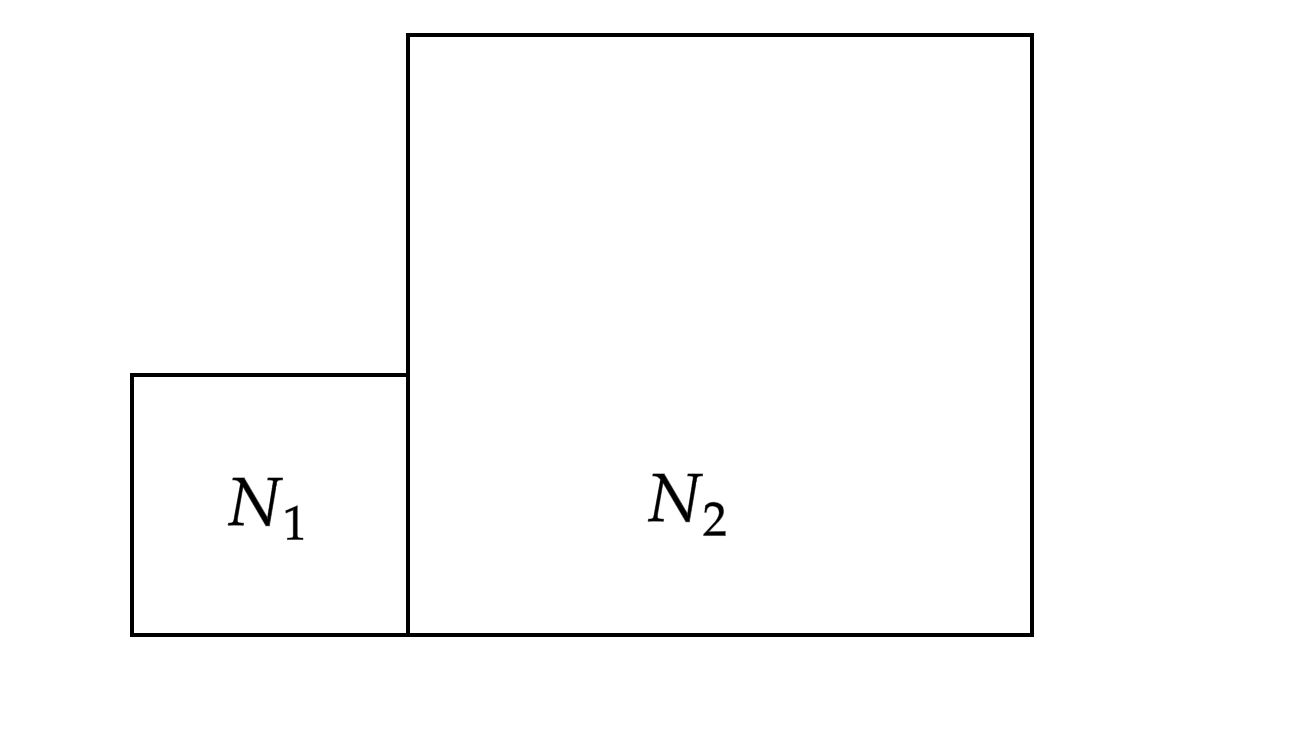
\includegraphics[width=0.5\textwidth]{fig/temperature.png}
       \caption{两个相互接触的热力学系统}
       \label{fig:temperature}
\end{figure}

因为\begin{equation}
       \di \Omega_1=\diffp*{{\Omega_1}}{{U_1}}{{N_1,V_1}}\di U_1 + \diffp*{{\Omega_1}}{{N_1}}{{U_1,V_1}}\cancelto{0}{\di N_1}+\diffp*{{\Omega_1}}{{V_1}}{{U_1,N_1}}\cancelto{0}{\di V_1}
\end{equation}
$\Omega_2$也是类似的,因此我们就有\begin{equation}
       \di \Omega=\Omega_1\diffp*{{\Omega_1}}{{U_1}}{{N_1,V_1}}\di U_1 + \Omega_2\diffp*{{\Omega_2}}{{U_2}}{{N_2,V_2}}\di U_2=0
\end{equation}
考虑到$U=U_1+U_2=\text{constant}$,因此$\di U_1+\di U_2=0$,所以\begin{equation}
       \di \Omega=\left(\Omega_2\diffp*{{\Omega_1}}{{U_1}}{{N_1,V_1}}- \Omega_1\diffp*{{\Omega_2}}{{U_2}}{{N_2,V_2}}\right)\di U_1=0
\end{equation}
从而
\begin{equation}
       \diffp*{{\ln \Omega_1}}{{U_1}}{{N_1,V_1}}- \diffp*{{\ln \Omega_2}}{{U_2}}{{N_2,V_2}}=0
\end{equation}
于是我们定义fundamental temperature $\tau =k_B T$满足\begin{equation}
       \frac{1}{\tau}=\diffp*{{\ln \Omega}}{{U}}{{N,V}}
\end{equation}
所以两个系统处于热平衡也就是\begin{equation}
       \tau_1=\tau_2
\end{equation}

从$\tau$的定义我们有\begin{equation}
       \Omega(U+\Delta U)=\Omega(U) e^{\frac{\Delta U}{\tau}}\quad\text{for}\ \Delta U\ \text{is small}
\end{equation}
于是当两个系统处于热平衡的时候,他们交换热量$\Delta U$\begin{equation}
       \Omega_1(U_1+\Delta U)\Omega_2(U_2-\Delta U)=\Omega_1(U_1) e^{\frac{\Delta U}{\tau}}\Omega(U_2)e^{-\frac{\Delta U}{\tau}}=\Omega_1(U_1)\Omega_2(U_2)
\end{equation}
这个关系要成立,$\Delta U$必须非常小。从这个关系我们可以发现温度可以表述成:系统的温度为$T$指的是,在平衡态附近当系统的能量增大一个$k_B T$的时候,系统的multiplicity function增大$e$倍。同时,因为$\Omega$依赖于$N,U,T$,所以只有对于平衡态才能够定义温度。



% section 温度 (end)
\begin{review}
     \item 遍历性假设
     \item 系综的基本概念
     \item 系统的状态参量
     \item 微正则系综及其应用
     \item mulltilicity function
     \item 温度的物理意义
\end{review}

\section{习题} % (fold)
\label{sec:习题1}
\begin{enumerate}
	\item Two systems, $A$ and $B$, of identical composition, are brought together and allowed to exchange both energy and particles, keeping volumes $V_A$ and $V_B$ constant. Show that the minimum value of the quantity $\left(\di  E_A / \di N_A\right)$ is given by
	$$
	\frac{\mu_A T_B-\mu_B T_A}{T_B-T_A}
	$$
	where the $\mu$ 's and the $T$ 's are the respective chemical potentials and temperatures.
	\item Making use of the fact that the entropy $S(N, V, E)$ of a thermodynamic system is an extensive quantity, show that
	$$
	N\left(\frac{\partial S}{\partial N}\right)_{V, E}+V\left(\frac{\partial S}{\partial V}\right)_{N, E}+E\left(\frac{\partial S}{\partial E}\right)_{N, V}=S .
	$$

	Note that this result implies that $(-N \mu+P V+E) / T=S$, that is, $N \mu=E+P V-T S$.

\end{enumerate}
% section 习题 (end)
% chapter 导言和系综理论基础 (end)
%---------------------------------------------------------------------------